In this chapter planning and work-flow regarding Sprint 1 will be described. 
All from setting our goals to implementation and testing. On the end we will evaluate whole sprint and try to answer on following questions: What went well? What could be improved? What should we start doing?  


\section{Sprint Planning}
After assembling all the tools in Sprint 0, we decided to start with the implementation of core modules.
As our understanding of task improved, we were able to come up with user stories from the perspective of user, customer, developer and student.
All user-stories were given to the customer so they can be prioritized. 
All but user-stories concerning our school obligations, like writing project plan, minutes, meetings with supervisor and attending lectures.
We decided to have school tasks as a user stories so we can better keep our time tracking. 
School user-stories were mandatory and already added as a user-stories of sprint 1.
On Monday 02.09.2013. we had the meeting with the customer where we estimated time we need for every user story.
Result of that meeting was list of rest of the user-stories for sprint 1.

For the documentation part, we made a document that we called the project plan, but the supervisor wanted these sections to be integrated in the project report instead. Therefore we decided to make the content for the report, and to make the general structure for it. Also integrate the parts we wrote in the project plan in the project report. We also plan to add the additional sections we need.

\subsection{Duration}
This Sprint will be 2 weeks long. From 02.09.2013 to 15.09.2013.
We agreed on the date for presentation and showing the running demo - Thursday 12.09.2013.
Estimated velocity is 240h since we agreed on 30 working hours per person per week.

\subsection{Sprint 1 User-stories}

All Sprint 1 user-stories are presented in table \ref{tab:sprint1stories}

\LTXtable{\textwidth}{sprint1/stories.tex}

\section{Sprint Goal}

Our goal for this Sprint is to deliver working demo over core client-server module.
This includes registering services, listening for the client and sending simple signals to the client from the server application.
Scanning for the services, connecting, receiving signals and play commands on the client.
Establishing simple communication protocol and implementing Test-Flight in both applications, the server and the client, is goal of this sprint too.

The goal for the documentation is to have a good structure for the report, and integrate the project plan in the project report. We need to evaluate if we need to write more of remove sections after integrating. The goal is also to finish the chapters that is a part of this sprint, which means we need to finish the sprint 0 chapter, and of course write the sprint 1 chapter.

\section{Architecture}

For the core communication and organization of our product we selected Client-Server Architecture \ref{fig:sprint1_arhitecture}.
Choosing this architecture was very intuitive to do as our project should consist of two applications and overall tasks should be partitioned. 
Client application should be able to light up different sequences of lights depending on server command signals.
And server application should be responsible for awaiting incoming clients connections, mapping clients to the grid and providing command play signals to the clients by broadcast.
Communication should be established over wireless network using same router for both applications, the user and the server, and without need for third party server nor Internet connection. 

\begin{figure}[H]
	\centering
		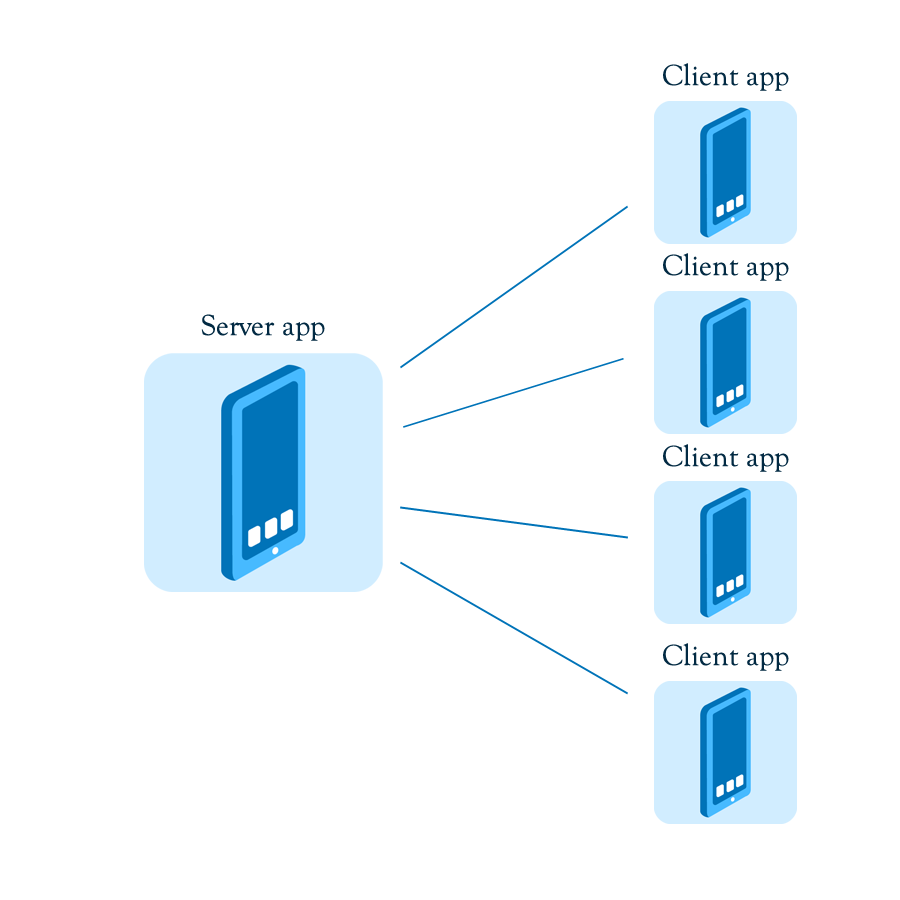
\includegraphics[width=7cm]{sprint1/arhitecture.png}
	\caption{Client-server architecture}
	\label{fig:sprint1_arhitecture}
\end{figure}

\subsection{"4+1" architectural view model}
For illustrating software architecture "4+1" architectural Model View\ref{fig:4+1 } will be used. It is based on the multiple concurrent views.

\begin{figure}[H]
	\centering
		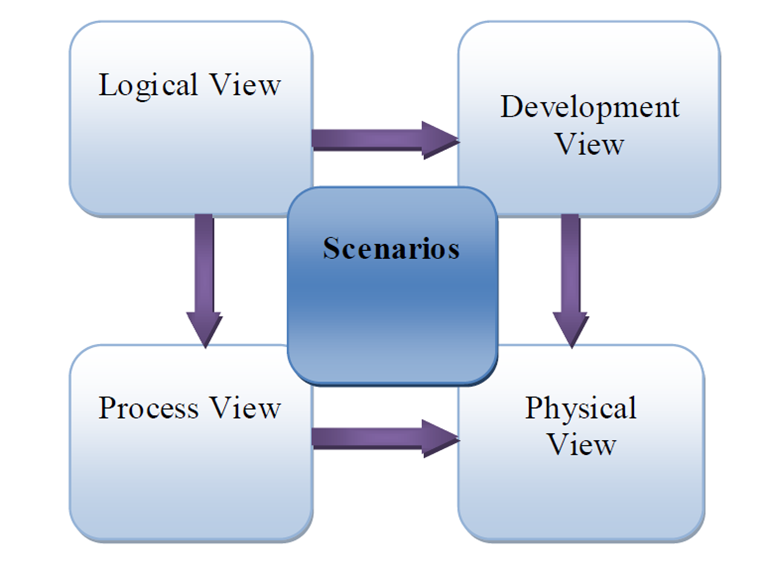
\includegraphics[width=7cm]{sprint1/4+1.png}
	\caption{"4+1" architectural view model}
	\label{fig:4+1 }

\end{figure}

\subsubsection{Logical View}
A description of the functional requirements of the architecture. The client and the server are decomposed into a set of key abstractions, taken(mostly) from the problem domain, in the form of objects or object classes.

Figure \ref{fig:class_diagram_client} gives an overview of the client class structure and collaboration. As planed client have all of the functionality covered by user stories. 

\begin{figure}[H]
	\centering
		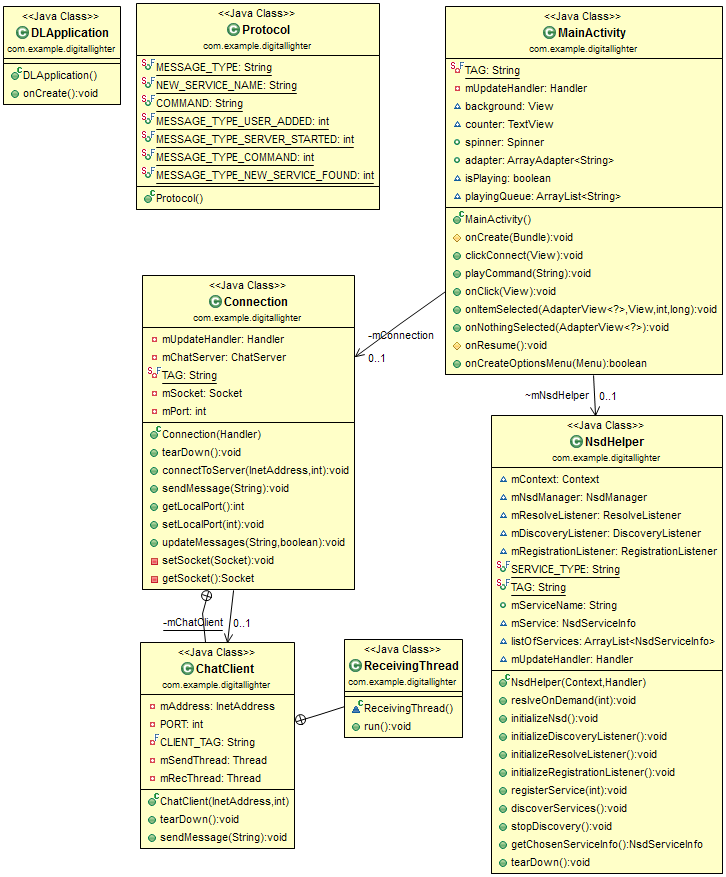
\includegraphics[width=10cm]{sprint1/class_diagram_client.png}
	\caption{Sprint 1 client class diagram}
	\label{fig:class_diagram_client}
\end{figure}

Figure \ref{fig:class_diagram_server} gives an overview of the server class structure and collaboration. We made separate thread "ServerThread" for incoming clients to optimize server. Sending command signals is also moved from ui thread to "SendingThread" in order to live more processing power for modules like image processing.

\begin{figure}[H]
	\centering
		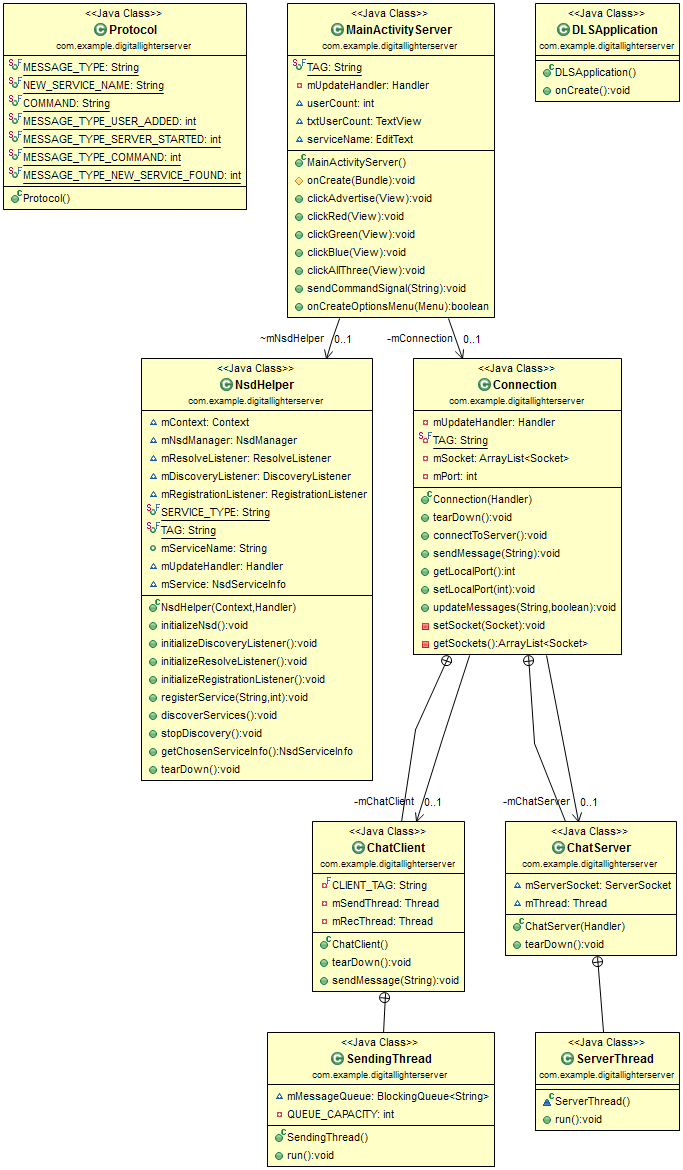
\includegraphics[width=10cm]{sprint1/class_diagram_server.png}
	\caption{Sprint 1 server class diagram}
	\label{fig:class_diagram_server}
\end{figure}

In the sequence diagram \ref{fig:sprint1_communication} is showed how applications can be used. It gives an idea of how the data flows between different parts of the system when it is up and running.

\begin{figure}[H]
	\centering
		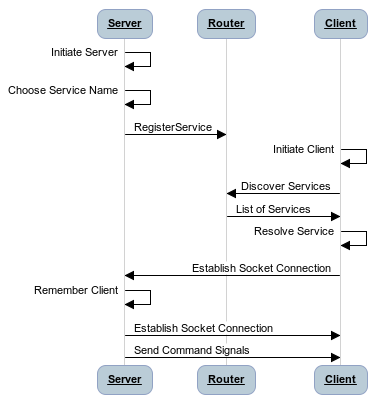
\includegraphics[width=9cm]{sprint1/communication.png}
	\caption{Sprint 1 Communication}
	\label{fig:sprint1_communication}
\end{figure}

\subsubsection{Physical View}
The deployment diagram, displayed in \ref{fig:deployment_diagram } describes the system architecture focusing on the large components and their connections.

\begin{figure}[H]
	\centering
		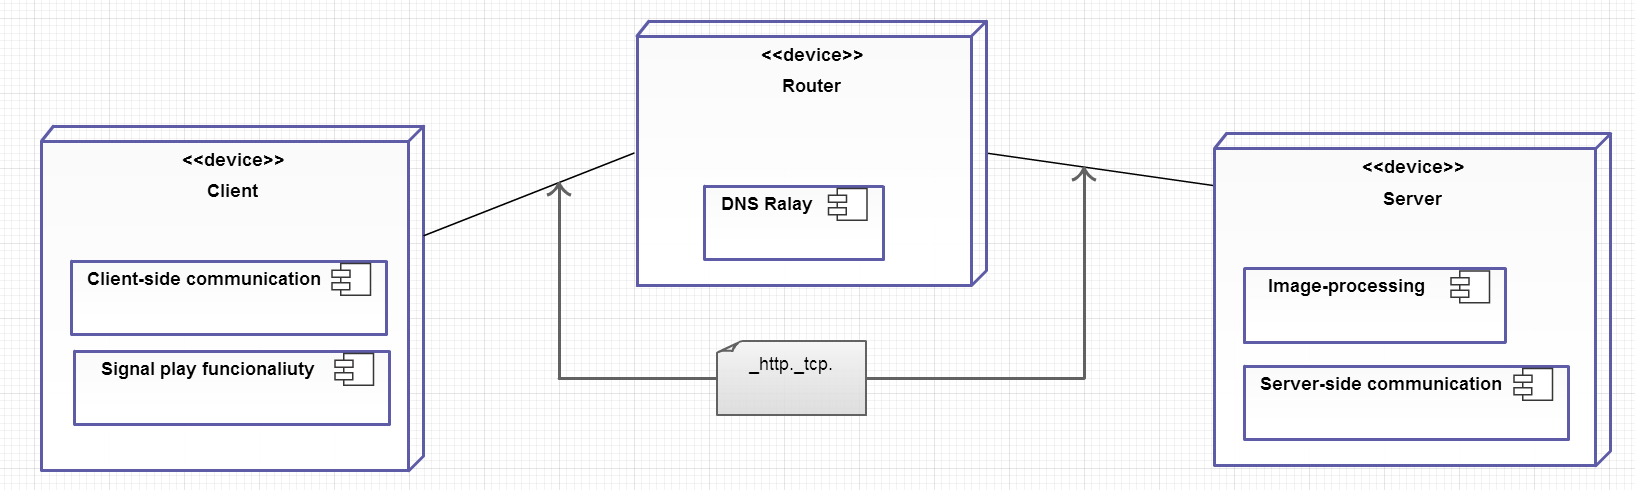
\includegraphics[width=15cm]{sprint1/deploy_diagram.png}
	\caption{Deployment diagram}
	\label{fig:deployment_diagram }
\end{figure}

\paragraph{Client}
is the application that runs on audience Android device. It is able to discover available services, connects to the one and receives command signals from the server. After receiving commands the client is able to flash screen according to given signal.

\paragraph{Router}
is inevitable part of client-server communication since our project is based on wireless network and zeroconf technologies. In order to support our demands it have to include a DNS relay. The relay embraces storing of service names and allows look-up stored data to the clients.

\paragraph{Server}
is the application that runs on manager's Android device. It have to register service that it provides at router DNS table. Once registered it have to be able to listen for the clients and broadcast command signals to them.

\subsubsection{Process View}

\subsubsection{Development View}

\section{Implementation}

Our first research of technologies that could help as at achieving client-server communication, without writing everything from scratch, was Bonjour software. 
It is the Apple's implementation of Zero configuration network (Zeroconf). 
Zero-configuration network (Zeroconf)  is a methodology and a set of special technologies that automatically create a usable computer network based on the Internet Protocol Suite (TCP/IP) when computers or network peripherals are interconnected. 
It does not require manual operator intervention or special configuration servers.
It is assembled of technologies that includes service discovery, addressing assignment, and host name resolution.
Aldo good and very useful tool it is not supported on Android, and since Android is our platform of choice we had to research further. 
We learned that we want zeroconf library with similar set of services as Bonjour written in Java.


Further research brought us to JmDNS. Java implementation of multi-cast DNS that can be used for service registration and discovery in Local Area Network. 
It works on most JDK1.6 compatible Virtual Machines, it comes as a library and it is easy to integrate with Android. 
JmDNS fulfill all of our expectations, but while learning about it over internet, we found that Android itself have built in Nestwork Service Discovery(NSD) that do the same thing.


Android Network Service Discovery(NSD) is supported from API version 16. 
It allows users to identify other devices on the local network, register services, broadcast connection information, scan for registered services and connect.
Even with minimum API limitation it is a part of Android platform, no third part libraries are needed, it will evolve with Android and therefore always be working.
Min API version was not of concern to the customer as he replied on mail regarding this question, so we made a decision of using Android Network Discovery(NSD) for client-server discovery and communication.

NSD send look like this:

Device Identifier: HelloWorldServer
Service Name: \_helloWorld.\_tcp.
Port: 27812
Network Address: 192.168.1.31

explain sockets

NSD
\section{Testing}

\section{Occurring risks}

That Android will not get NSD able for low APIs. 
Then we have to use third part libraries.

\section{Retrospective and Evaluation}
In this section the team will take a look back at sprint 1, and review this sprint. The focus will be on what went well, and goal we achieved. Another focus will also be what we could have done differently, and of course and learn from what we could have done differently.

Obedient client - Prototype 1
 Put "Hello World" project to gitHub and pull it to every group members
local storage.
 Set up protocol for client & server.
 Make server able to listen for clients.
 One client connects to the server.
 The server sends command to one client.
 The client receives one command.
 The client "plays" one command (white light 10 seconds).

The customer was very satisfied with the video for sprint 1, and suggested recording our future prototypes as well. 
Planning.

\subsection{Pros}
The team reached the sprint 2 goals. The team delivered the demo with our more refined code, and as planned this code supported multiple clients. The clients were able to play the commands the server sent. We also reached the milestone, Obedient crowd - Prototype 2.
\subsection{Cons}

Create sequence diagram (flow diagram) for architecture section.
report
Improve connection between user stories and requirements
Structure and organize the sprint user stories
WBS
Finished:
Reduce number of chapters in report
